\chapter{Regularisation of Models}
\label{ch:regularisation-of-models}\index{regularisation-of-models|(}


\section{Introduction}


\textit{Regularisation of Models} deals with the widespread problem of overfitting in machine learning (ML) models. When a ML model is overfitting it implies that the model has been trained in such a way to perform well on the particular training data but performs badly when using test or unseen data. The overfitting model learns the pattern as well as the noise in the training data. This can be caused when the model has a high variance and when the model is highly complex with respect to the underlying data. The other extremity is underfitting where the model has a high bias. These are illustrated in Figure~\ref{fig:rom_overfitting} where the underfitting model is represented by a low degree polynomial ($y = x$) with respect to the underlying data, and the overfitting model is represented by a high degree polynomial ($y = x^{n}$) \citep{pythonmachinelearning}. High variance refers to the variability of the model output prediction for test inputs that were not used during training and represent the overfitting case, whereas high bias refers to the errors due to the `assumptions` of the model that differ from the actual, since the model does not reflect the underlying relationship of the data. The challenge is to find a good bias-variance trade-off.

\begin{figure}
  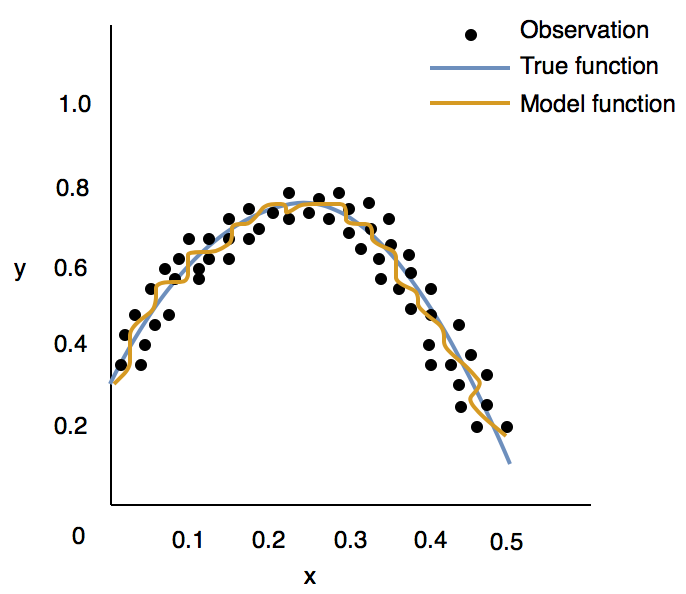
\includegraphics{regularisation_of_models/overfitting.png}
  \caption{Overfitting and Underfitting: Challenge for a good bias-variance trade-off (Adapted from\citet{pythonmachinelearning}). }
  \label{fig:rom_overfitting}
\end{figure}


The \textit{compromise} or \textit{generalisation} challenge can be tackled using regularisation techniques. A number of regularisation techniques will be discussed in this chapter including i) L1 regularization, ii) L2 Regularization, iii) Dropout, and iv) Early Stopping.


\section{L2 and L1 regularization} \index{L2 and L1 regularization}


Regularization is a technique that alters the learning algorithm to add noise during the learning process in such a way that the model can generalise better. This generalisation is achieved by introducing a bias so that an overfitting model achieves bias-variance compromise as illustrated in Figure~\ref{fig:rom_overfitting}. The learning algorithms such as regression and deep learning typically learn using a cost or error function which is minimized such that the model with minimum error is determined. Regularisation uses a \textit{regularisation} parameter $\lambda$ to add the bias or penalty to the error function as the model complexity increases. Function \ref{eq:rom_penalty}  defines a simplified loss/cost function with regularisation.

\begin{equation}
\label{eq:rom_penalty}
minimize ( cost function, c(x) + \lambda(penalty function) )
\end{equation}

Function  \ref{eq:rom_penalty} includes two terms; i) the cost function, and ii) the penalty (regularization) function, where the penalty function is constrained to be less than or equal to a constant, t \citep{friedman2001elements}.

To train the model, minimisation is done on both the cost and penalty functions. The cost function, c(x) depends on the training data whereas the regularisation function is independent of the data variable ($x_n$). Parameter $\lambda$ is determined empirically or through cross validation, and it is used to control how to balance out the two terms in function \ref{eq:rom_penalty}  by balancing how much the model should learn the training set, and how much bias to add. There are two methods for regularisation that apply a bias which are termed L2 and L1, known as Ridge \index{Ridge Regression} and Lasso Regression \index{Lasso Regression} respectively. L2 and L1 penalize weights differently.




\subsection{L2 Regularisation} \index{L2 and L1 regularization!L2 Regularisation}


L2 regularisation penalizes the $weight^2$. Therefore, considering the cost function for linear regression as an example, function \ref{eq:rom_penalty} can be re-written as:

\begin{equation}\label{rom_l2}
minimize ( \sum^{n}_{i=1}(y_i - w_0 - \sum^{p}_{j=1}(x_ij.w_j) )^2 + \lambda\sum^{p}_{j=1}(w_j^2) )
\end{equation}

Where $y_i$ is the predicted value from which the actual value is subtracted. The weight, ($w_0$) (intercept in linear regression) is left of out the penalty function. In L2 regularisation $\lambda$ is a complexity parameter that controls the amount of shrinkage \citep{friedman2001elements}.  The idea of penalizing by the $weight^2$ is also used in neural networks where it is known as weight decay \citep{krogh1992simple,moody1992effective}. \citet{krogh1992simple}, claim that the ``generalisation ability of a Neural Networks depend on a balance between the information in the training example and the complexity of the network``, where the complexity is related to the number of weights in the model. L2 regularisation tries to minimize the number of weights, and therefore make the model less complex (decrease the polynomial degree), whilst still minimizing the error. 


\subsection{L1 Regularisation} \index{L2 and L1 regularization!L1 Regularisation}


On the other hand, L1 penalizes on the |weight| \citep{friedman2001elements}. Therefore the function is rewritten as:

\begin{equation}\label{rom_l1}
minimize ( \sum^{n}_{i=1}(y_i - w_0 - \sum^{p}_{j=1}(x_ij.w_j) )^2 + \lambda\sum^{p}_{j=1}(w_j) )
\end{equation}

The derivative of L2 and L1 regularisation term would result in $2w$ and $k$ (a constant) respectively (considering penalty function only), when computing partial derivatives with respect to the weights, ($w_n$). Therefore, L2 regularisation removes a percentage from the weight, whereas L1 subtracts a constant from the weight. This creates a significant difference from the Ridge function as it will cause some of the coefficients to be exactly zero for an appropriate value of t \citep{friedman2001elements}. L2 regularization pushes less important weights towards zero however it does not force them to be exactly zero.

\citet{ng2004feature} considered supervised learning problems where the feature space is made up of many irrelevant features (noisy), and studied L1 and L2 regularization applied on logistic regression methods for preventing overfitting. L1 regularisation cause the weights of some features to go to zero, making it highly suitable for models where many of the features should be ignored. He has found L1 regularisation to be effective in these scenarios and concluded that L1 regularized logistic regression can be effective even if there are exponentially many irrelevant features as there are training examples.


Since L1 regularisation encourages the weight for meaningless features to drop to exactly zero, consequently being removed from the model, it makes this technique suitable for sparse datasets where there could be potentially considerable meaningless features or dimensions. On the other hand L1 regularisation can have the negative affect that it zeros the weight for weakly informative dimensions. 


\section{Dropout} \index{Dropout}

Dropout is another regularisation technique that is targeted for neural networks (NN) models and was proposed by \citet{srivastava2014dropout}. The dropout techniques adds bias or noise to the NN model in order to prevent overfitting similar to the L1 and L2 regularisation techniques described earlier. In order to add this bias, the dropout technique removes nodes together with their input and output connections randomly during training. The Dropout technique is illustrated in Figure~\ref{fig:rom_dropout_a},\ref{fig:rom_dropout_b}. 

\begin{marginfigure}%
	\centering
	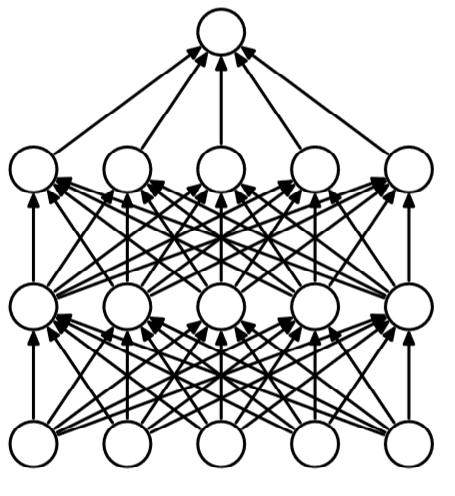
\includegraphics[width=\linewidth]{regularisation_of_models/dropout_a.png}
	\caption{Standard Neural Net (Reproduced from \citet{srivastava2014dropout}).}
	\label{fig:rom_dropout_a}
\end{marginfigure}


The random dropout action is performed during the training phase only, and it creates a different thinned NN (Figure~\ref{fig:rom_dropout_b}) \index{Thinned Neural Network} for each epoch. Therefore the minimisation, through back propagation, of the NN loss function is only applied to the thinned network, and the inactive neurons do not participate in the training of that epoch. The intensity of the dropout is regulated by hyperparameter $p$, describing the probability of retaining a unit, where $p = 1$ implies no dropout. Dropout can be applied both for the input layer, and also on each of the hidden layers. \citet{srivastava2014dropout} have determined that the typical values of \textit{p} for hidden layers is between $0.5-0.8$, whilst for real-valued inputs $0.8$ is used. Choosing an incorrect value of \textit{p} can induce too much bias and may lead to underfitting

\begin{marginfigure}%
	\centering	
	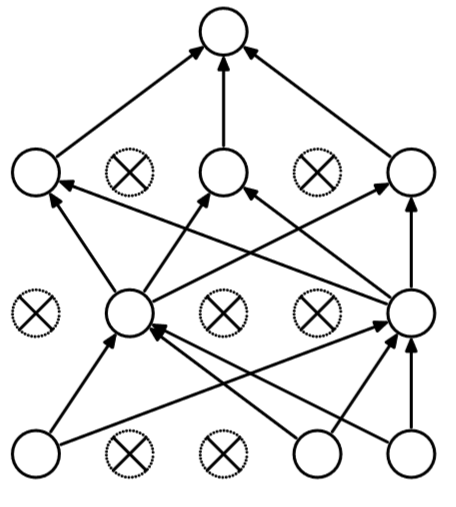
\includegraphics[width=\linewidth]{regularisation_of_models/dropout_b.png}
	\caption{Thinned Neural Net after applying dropouteproduced from \citet{srivastava2014dropout}).}
	\label{fig:rom_dropout_b}
\end{marginfigure}



During each training epoch a \textit{masking} vector is created using the probability \textit{p} applied on a \textit{Bernoulli Distribution}, where its output is either 1 or 0 to determine which neurons are activated. Therefore considering a layer of $n$ neurons, $(1-p) \times n$ neurons would be masked at each epoch. 

At the end of the training each node would have been trained a different number of times, however each epoch contributes to the same sets of weights. On the other hand, during the testing phases dropout is not utilised and all the neurons are again active. However, before testing, the weights obtained from the different thinned networks are further penalized by multiplying each outgoing weight with the probability \textit{p} that was used during testing.

\citet{srivastava2014dropout} et al have determined that dropout was successful in various domains including speech recognition and document classification to mention a few. The authors have concluded that the dropout method is a general technique that can be applied across different domains, however it has the drawback of extending the training time by typically $2-3$ times.


\section{Early Stopping} \index{Early Stopping}



Early Stopping is a method applied to NN where the training model is stopped before the training error is minimized \citep{Sarle95stoppedtraining}.Figure~\ref{fig:rom_early} illustrates a typical plot of the accuracy of model versus the epochs for the `Training Data` and `Test Data`. At each iteration the test data is used to evaluate out the model being trained. As can be noticed although the training accuracy continues to increase as cost function is minimized, the `Test Data` accuracy start dropping after a certain epoch.

\begin{marginfigure}%
	\centering
	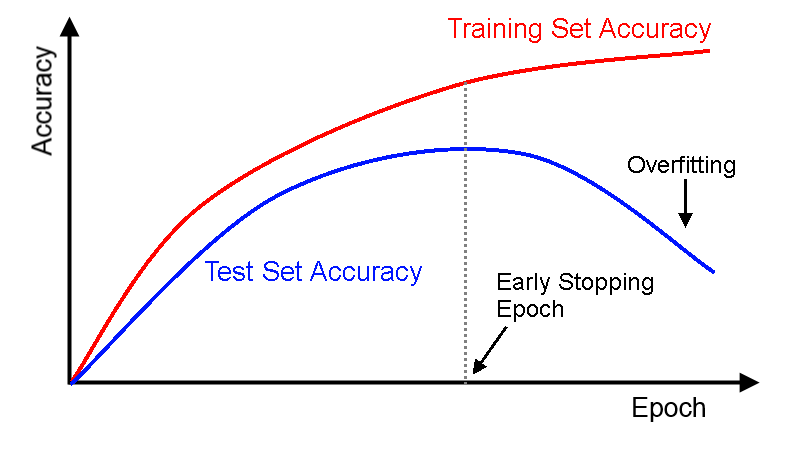
\includegraphics[width=\linewidth]{regularisation_of_models/earlystopping.png}
	\caption{Training Data Accuary Vs Test Data Accuracy}
	\label{fig:rom_early}
\end{marginfigure}

Early Stopping determines the number of epochs a model is allowed to run by evaluating the  \textit{training} model after each epoch (or $n$ epochs). The model is stopped if subsequent training results in lower performance. This marks the `Early Stopping Epoch` as shown in Figure~\ref{fig:rom_early}. \citet{zur2009noise} showed that early stopping reduces the effect of overfitting but is it is not as effective as weight decay using L1 and L2 regularisation. Early Stopping is considered a form of regularisation method since it helps the model from overfitting.



\index{Regularisation of Models|)}
